\documentclass[paper=a4, fontsize=11pt]{scrartcl} % A4 paper and 11pt font size
\usepackage[T1]{fontenc} % Use 8-bit encoding that has 256 glyphs
\usepackage{fourier} % Use the Adobe Utopia font for the document - comment this line to return to the LaTeX default
\usepackage[english]{babel} % English language/hyphenation
\usepackage{amsmath,amsfonts,amsthm} % Math packages
\usepackage{sectsty} % Allows customizing section commands
\allsectionsfont{\centering \normalfont\scshape} % Make all sections centered, the default font and small caps
\usepackage{fancyhdr} % Custom headers and footers
\pagestyle{fancyplain} % Makes all pages in the document conform to the custom headers and footers
\fancyhead{} % No page header - if you want one, create it in the same way as the footers below
\fancyfoot[L]{} % Empty left footer
\fancyfoot[C]{} % Empty center footer
\fancyfoot[R]{\thepage} % Page numbering for right footer
\renewcommand{\headrulewidth}{0pt} % Remove header underlines
\renewcommand{\footrulewidth}{0pt} % Remove footer underlines
\setlength{\headheight}{13.6pt} % Customize the height of the header
\numberwithin{equation}{section} % Number equations within sections (i.e. 1.1, 1.2, 2.1, 2.2 instead of 1, 2, 3, 4)
\numberwithin{figure}{section} % Number figures within sections (i.e. 1.1, 1.2, 2.1, 2.2 instead of 1, 2, 3, 4)
\numberwithin{table}{section} % Number tables within sections (i.e. 1.1, 1.2, 2.1, 2.2 instead of 1, 2, 3, 4)
\setlength\parindent{0pt} % Removes all indentation from paragraphs - comment this line for an assignment with lots of text

\usepackage{xcolor}
\usepackage{graphicx}
\usepackage{listings}
\lstset{
  basicstyle={\small\ttfamily},
  keywordstyle={\bfseries\color{NavyBlue}},
  breaklines=true,
  emphstyle={\bfseries\color{Rhodamine}},
  commentstyle={\color{PineGreen!60!black}},
  stringstyle={\rmfamily\color{YellowOrange}},
  showstringspaces=false,
  frame=shadowbox,
  breakatwhitespace=false,
  captionpos=b,
  extendedchars=true,
  keepspaces=true,
  numbers=left,
  numberstyle=\tiny,
  rulecolor=\color{black},
  rulesepcolor={\color{blue!20!white}},
  showspaces=false,
}

\newcommand{\horrule}[1]{\rule{\linewidth}{#1}} % Create horizontal rule command with 1 argument of height

\title{	
\normalfont \normalsize 
\textsc{Final Team Report for ``Human Computation'', Summer Term 2017, IFI LMU} \\ [25pt]
\horrule{0.5pt} \\[0.4cm] % Thin top horizontal rule
%%
%% TITEL
%%
\huge Final Team Report for HC System: \\
Designing and Implementating A GWAPs Disaster Monitoring System\\%edit as appropriate
\horrule{2pt} \\[0.5cm] % Thick bottom horizontal rule
}
\author{\\ Team: Hotpot\\Changkun Ou : <11406972> \\Yifei Zhan : <Matrikelnummer> \\Zhe Li : <Matrikelnummer>  }
\date{\today}

\begin{document}

\maketitle % Print the title

\tableofcontents

\paragraph{Abstract}

Abstract test

\section{Introduction}
Introduction cite test \cite{Bry2013} 

\section{Related Work}
  \subsection{Human Computation}
  \subsection{Human-Computer Interaction}
  \subsection{Network Analysis}

\section{The Disaster Monitoring System}

  \subsection{Game Design}
    \subsubsection{User Motivation}

    A player can finish infinity Round tasks, 
    a Round task contains {N} tagging tasks, 
    the player tagging task is to:

    \begin{itemize}
      \item Select a Region Of Interests(ROI) upon the presented satellite image;
      \item Tag the ROI from a provided tag list or input their own tag, the provided tag list contains: $T_1, T_2, …, T_n, \text{other(input needed)}$
    \end{itemize}

    Note that:

    \begin{itemize}
      \item A ROI is a sub-rectangle-window of a image;
      \item Multiple selections;
      \item Anyone can directly participant without registration, but system records an ID
    \end{itemize}

    \subsubsection{User Work-flow}

  \subsection{Aggregation Model and System Design}

    \begin{figure}[htp]
    \centering
    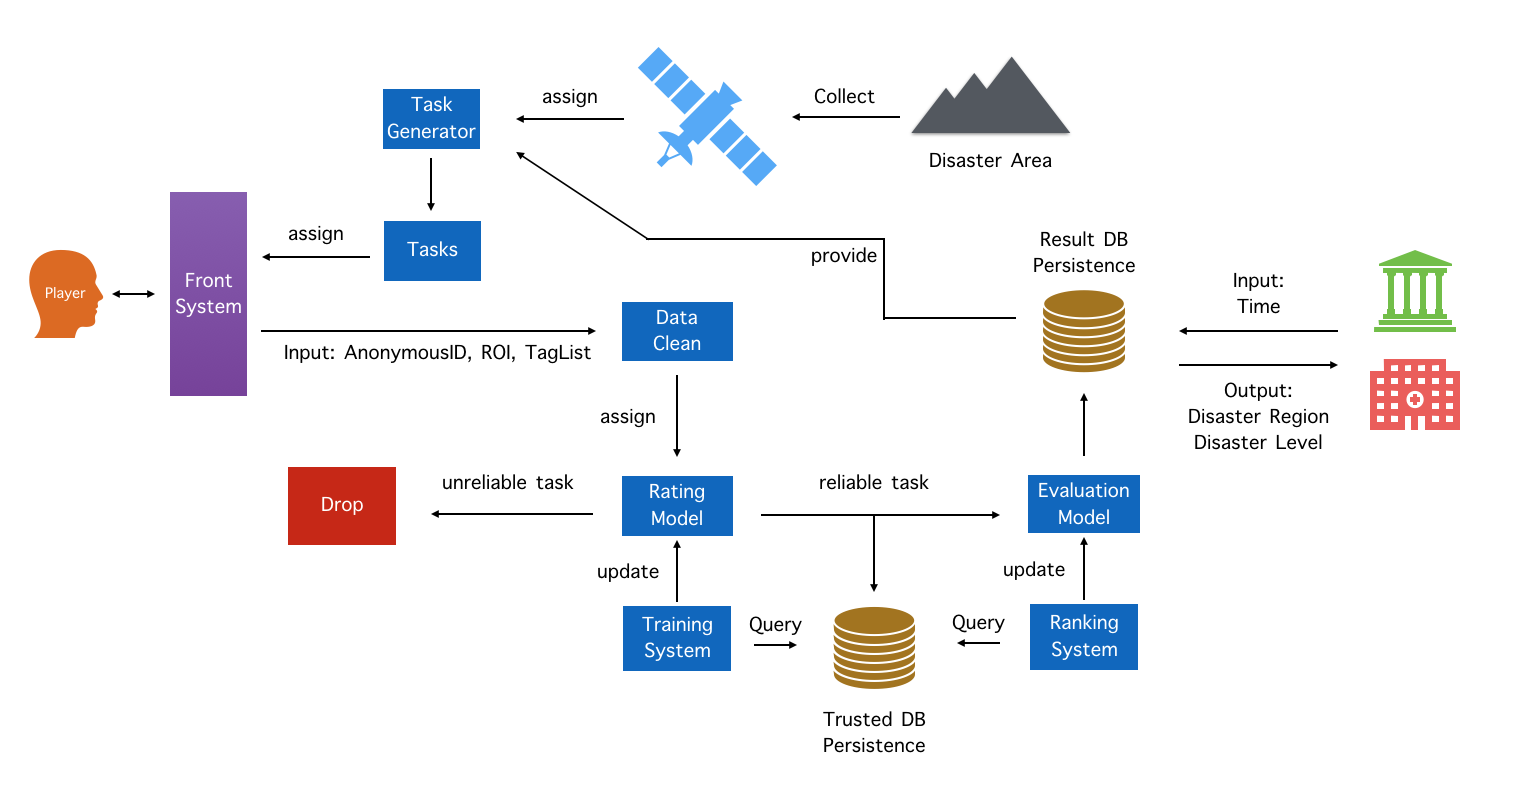
\includegraphics[width=\textwidth]{figures/system}
    \caption{System Design Overview}
    \label{fig:roiweight}
    \end{figure}

    \subsubsection{Task Generator}

    A task generator combines images from satellite and Result DB:

    \begin{itemize}
      \item Split a certain monitoring area image to pieces of images;
      \item Mix images from Result DB and pack as a Tagging Task which to be assigned to player.
    \end{itemize}

    \subsubsection{Player Rating Model}

    Player’s input vector: 
    
    \[
    (\text{anonymous\_id}, \text{image}, \text{event\_time}, \text{ROI}, \text{tag\_list})
    \]

    Model output: 
    
    \[
    (\text{anonymous\_id}, \text{trust\_value})
    \]

    Note that:

    \begin{itemize}
      \item $(anonymous\_id, image, event\_time, ROI)$ is the primary key of the input vector;
      \item A player can generate multiple vectors to rating system even for same image;
      \item The event\_time is the capture time of the satellite image.
    \end{itemize}

    \begin{figure}[htp]
    \centering
    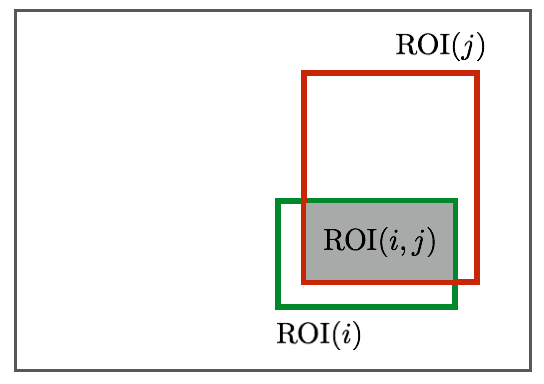
\includegraphics[width=4cm]{figures/weight-define}
    \caption{Weight Definition Visualization}
    \label{fig:roiweight}
    \end{figure}

    For a certain image $img$ at time $t$, Rating: player $i$ $\rightarrow$ player $j$:

    \[
    w_{ij}=\sum_{\text{ROI}\in \text{ROIs}}\frac{\text{ROI}(i,j)}{\text{ROI}(i)} \times \frac{Cov(\text{tags}(i), \text{tags}(j))}{\text{var}(\text{tags}(i))\text{var}(\text{tags}(j))} \geq 0
    \]

    Normalized Adjacency Matrix:

    \[
    A = (\frac{w_{ij}}{\sum_{j}{w_{ij}}})
    \]

    Obviously, A is \textbf{irreducible, real, non-negative, column-stochastic, and diagonal element being positive,} then eigenvalue of A is the player trust value.

    When a new player tagging task need to be rated,

    \begin{itemize}
      \item which means we need introduce a new node to the graph
      \item need calculate the trust value of new graph
      \item let $t’$ is the trust value of new player
      \item if $t’ >= \text{mean}(\text{old\_eigenvalues})$, then it is a reliable player, otherwise drop it.
    \end{itemize}

    \subsubsection{Disaster Level Evaluation Model}

    Query input:

    \[
    (\text{time}) or (\text{area\_id})/(\text{area\_id}, \text{time})
    \]

    Model output:

    \[
    (\text{area\_id}, \text{time}, \text{disaster\_level})
    \]

    Note that:

    \begin{itemize}
      \item All results are evaluated from reliable tasks
      \item Evaluation Model generated by all reliable history
    \end{itemize}

    Now we have trusted results, each area has its tagging history.

    For an area at time t, define disaster level as follows:

    \[
    v_{area} = \frac{
    \sum_{\text{tag}\in\text{tags}}
      {w_{tag}\times\#(\text{tag})}
    }
    {\sum_{area\in areas}{\sum_{\text{tag}\in\text{tags}}{w_{tag}\times\#(\text{tag})}}}
    \]

    where $w_{tag}$ is pre-defined weight by system, $\#(tag)$ is the occur number of a tag.

    Return value:

    \begin{itemize}
      \item disaster region: $\cup_{ROI\in ROIs}{ROI}$
      \item disaster level: $v_{area}$
    \end{itemize}

    \subsubsection{Data Persistence}

    Trusted DB Fields:

    \begin{lstlisting}[
      caption={Trusted Database Field},
      label={lst:trustdb}
    ]
    [
        {
            "anonymous_id": number,
            "tasks": [
                {
                    "image": image_path,
                    "at_time": time, 
                    "ROI": [
                        {
                            "latitude": number,
                            "longitude": number,
                            "tags": [tag1, tag2, ...]
                        }
                    ]
                }
            ]
            "trust_value": number
        }
    ]
    \end{lstlisting}

    Result DB Fields:

    \begin{lstlisting}[
      caption={Results Database Field},
      label={lst:resultdb}
    ]
    [
        {
            “area_id": number,
            "history": [
                {
                    “at_time”: time,
                    "image": image_path,
                    "ROI": [
                        {
                            "latitude": number,
                            “longitude": number,
                            "tags": [tag1, tag2, ...]
                        }
                    ],
                    "disaster_level": number
                }
            ]
        }
    ]
    \end{lstlisting}

    \subsubsection{TL; DR}

    \begin{itemize}
      \item Task Generator combines trusted results assign to players;
      \item Always treat player as new player, but integrated as old player if exists;
      \item Use ROI matching rate as graph edge weight, eigenvalue as trust value of player;
      \item Disaster Evaluation use pre-defined weight, then defined the disaster level
    \end{itemize}

\section{Prototype}

  \subsection{Requirements Selection}
  For a prototype, we decided to use the following framework to implement everthing:

  \begin{itemize}
    \item Polymer
    \item Node.js
    \item MongoDB
  \end{itemize}
  \subsection{Front End}
  \subsection{Back End}

\section{Discussion}

  \subsection{Model Evaluation}
  \subsection{Issues on Social Aspects}
  \subsection{Issues on Ethical Aspects}

\section{Conclutions}

In this report, we present a disaster monitoring system, which aggregate human tagging input based on
Network Analysis. 

\nocite{*}
\bibliographystyle{plain}
\bibliography{ref}

\end{document}
